\documentclass[11pt,a4paper]{article}
\usepackage[T1]{fontenc}
\usepackage{lmodern,microtype}
\usepackage[margin=0.85in]{geometry}
\usepackage{amsmath,amssymb,amsthm,mathtools}
\usepackage{booktabs,tabularx,array,enumitem,needspace,float}
\usepackage{flafter}
\usepackage{xcolor,tikz}
\usetikzlibrary{arrows.meta,positioning,calc,decorations.pathreplacing}
\usepackage[hidelinks]{hyperref}
\setlength{\parindent}{0pt}
\setlength{\parskip}{4pt}
\setlength{\emergencystretch}{2em}
\setlist{nosep,leftmargin=*}
\newcolumntype{Y}{>{\raggedright\arraybackslash}X}
\newcolumntype{P}[1]{>{\raggedright\arraybackslash}p{#1}}
\theoremstyle{definition}
\newtheorem{definition}{Definition}[section]
\newtheorem{assumption}[definition]{Assumption}
\numberwithin{equation}{section}
\newcommand{\Hash}{\mathsf H}
\newcommand{\QC}{\mathsf{QC}}
\newcommand{\FC}{\mathsf{FC}}
\newcommand{\TB}{\mathrm{TB}}
\newcommand{\tagg}[1]{\mathsf{#1}}
\definecolor{rrBlue}{HTML}{2563EB}
\definecolor{rrTeal}{HTML}{0F766E}
\definecolor{rrOrange}{HTML}{B45309}
\title{Regional Sequencer Rotation\\Draft Sections 2 and 3}
\author{}
\date{25 October 2026}
\begin{document}
\maketitle
\setcounter{section}{1}
\section{Model, Assumptions, and Goals}
\label{sec:model}

This section states the external conditions under which the protocol is
studied and the properties its construction must establish.  L1 and
Espresso are sources of finalized data; their internal consensus
protocols are outside the model.  The rotation, publication, and recovery
rules remain part of the protocol being specified.

\subsection{Participants, time, and failures}
\label{sec:model-participants}

% P-2.01
The system serves one L2 chain under a fixed chain identifier and rule
version.  Its registered regions are denoted by $\mathcal L_R$.  Users
submit ordinary transactions to block builders.  Stakers register
operator keys and escrow through the L1 Authority, which also records
multisignature controls.  Regional replicas run session programs; a
session $s=(\beta,r)$ is one regional turn on branch version $\beta$.
Publishers relay complete regional results to Espresso.  Batchers submit
the corresponding batch data through a trusted certifier and the L1
inbox.  External observers either follow public finality directly or
derive the L2 chain from finalized L1 inputs and DA data.  These are
logical roles: one operator may perform several of them.  Precise
identifiers and shared objects are defined in
Section~\ref{sec:shared-objects}.

Real time is denoted by $\tau$; $t$ is reserved for a leader term.  An L1
block has height $\ell$, and its transactions and events have a fixed
order.  Espresso block $J_q$ has height $q$ and timestamp $\theta_q$.
These source coordinates are distinct from L2 block height and from the
time at which a particular observer receives data.  A global clock
provides a common interpretation of local protocol deadlines without
requiring simultaneous receipt of messages or source records.

% P-2.02
The adversary may control regional participants up to the weight bound
below, send arbitrary messages, and schedule deliveries within the
applicable communication bounds.  The recovery model additionally
allows Espresso to stop finalizing new blocks.  Such an outage suspends
the healthy-period Espresso progress guarantees, while its previously
finalized history remains consistent and immutable.  Availability of
historical bytes is a separate condition.  This model does not include
conflicting finalized Espresso histories, failure of L1 finality, or a
compromised trusted certifier.

\subsection{External assumptions}
\label{sec:external-assumptions}

All service bounds in this subsection apply within the declared
admission, input-size, and load limits, with the required fee resources
and working submission routes.  Their consumers are correct
participants that remain online and keep up with the relevant history.
A request is \emph{submitted} when the complete request reaches the
service's admission boundary, rather than when a node attempts a local
send.  Bounds that include visibility cover dissemination, retrieval,
and the specified verification work as well as finalization.

% P-2.03 / AS-01
\Needspace{7\baselineskip}
\begin{assumption}[Finalized L1 history and service]
\label{ass:l1}
\textup{(S)} Authenticated finalized L1 prefixes are mutually compatible
and persistent.  They determine the same transaction order, execution
outcomes, events, and contract state at each finalized height.  A
consumer can authenticate the exact contents and completeness of a
specified range of relevant records, including an empty range.  L1
faithfully executes the deployed contract code.

\textup{(L)} There is a bound $T_{\rm L1}>0$ such that an admitted L1
operation actually submitted at time $\tau$ has a finalized execution
result by $\tau+T_{\rm L1}$, and by then the result is retrievable and
verifiable by the consumers specified above.  A finalized result may
report success or failure: state-dependent competing calls are not all
guaranteed to succeed.
\end{assumption}

The authenticated state includes Authority snapshots, bans, recovery and
closure records, the control log, and the inbox's acceptance and mode
events.  A selected collection of individually valid events does not
establish a complete control prefix.  The L1 bound begins at actual
submission and excludes fault detection, governance deliberation, and
signature collection beforehand.

% P-2.04 / AS-02
\Needspace{7\baselineskip}
\begin{assumption}[Finalized Espresso history and healthy-period service]
\label{ass:espresso}
\textup{(S)} Finalized Espresso blocks form one persistent, publicly
verifiable history.  Each block determines the complete ordered content
of this chain's namespace, including authenticated absence of content.
Its timestamps are non-decreasing.  If $J_q$ first becomes final at real
time $\tau_E(q)$, then, for a fixed $\epsilon_E\ge0$,
\begin{equation}
\label{eq:espresso-clock-lead}
 \theta_q\le\tau_E(q)+\epsilon_E.
\end{equation}

\textup{(L)} For a fixed $T_E>0$, if Espresso remains healthy throughout
$[\tau,\tau+T_E]$, an admissible complete publication actually submitted
at time $\tau$ is finalized and visible to the specified consumers by
$\tau+T_E$.  Every newly
finalized block, including an empty relevant namespace, is retrievable
and verifiable within $T_E$ of finalization under the same service
conditions.  If Espresso remains healthy, finalized block heights and
timestamps progress without bound.
\end{assumption}

Clause~(S) continues to hold in the outage model.  Clause~(L) is not used
to bound a new publication during an outage.  Finalized inclusion fixes
the published bytes and their source positions; application validity
and permission to extend the global chain are decided by this
protocol.  The timestamp condition bounds clock lead, but does not
identify a block's finalization time with its timestamp or supply a
bound on arbitrary historical retrieval.

% P-2.05 / AS-03
\Needspace{7\baselineskip}
\begin{assumption}[Authenticated synchronous communication and clock]
\label{ass:communication}
Participants share a global clock and use authenticated communication.
A complete message sent between correct, operational members of region
$i$ is delivered and processed within $\Delta_i$.  A complete message
sent between correct, operational endpoints in different regions is
delivered and processed within $\Delta_{\rm cross}$ through the mixed
peer-to-peer backbone.  These bounds apply to the declared message and
validation-dependency sizes and processing budgets; the backbone has a
working correct route under its stated fault conditions.
\end{assumption}

Messages may be duplicated or delivered out of order, and a Byzantine
sender may remain silent.  Authentication establishes the sender and
bytes, not the truth of the sender's claim.  The bounds include the
validation and state-adoption work expressly covered by a complete
message.  Any additional state reconstruction or installation has its
own preparation budget.  In particular, synchrony does not make an
unprepared recipient Ready, and a source record need not become known
to every replica at the same instant.

% P-2.06 / AS-04
\Needspace{7\baselineskip}
\begin{assumption}[Cryptography and fixed-committee faults]
\label{ass:regional-faults}
Signatures of uncompromised keys cannot be forged, and hashes bind their
canonically encoded inputs.  Session $s$ has a fixed committee $V_s$
with positive integer voting weights $w_o$, total weight
$W_s=\sum_{o\in V_s}w_o$, and fault bound $0\le F_s<W_s/2$.  The total weight
of committee keys controlled by Byzantine participants, including later
key compromises, over the period in which their
certificates may authorize new output is at most $F_s$.  Historical
certificates retain these weights; neither a later slash nor a later
configuration reweights them.
\end{assumption}

Every regional certificate requires matching signatures from distinct
members of total weight strictly greater than $F_s$.  Consequently it
contains a correct signer, and the correct members have enough total
weight to form a certificate themselves because $W_s-F_s>F_s$.
These facts do not assert honest intersection between arbitrary pairs
of certificates.  Regional safety also uses the synchronous forwarding,
timer, and recovery-lock rules.  The accepted-lifetime restriction is
essential when interpreting old signatures.  Subsequent old-key
compromise outside that lifetime is outside this analysis.  Stake
registration alone does not establish the assumed fault bound.

% P-2.07 / AS-05
\Needspace{7\baselineskip}
\begin{assumption}[DA, retention, and state preparation]
\label{ass:data-state}
A valid DA commitment binds the exact submitted payload under the fixed
DA encoding and verification rules.  Under the specified availability
and retention conditions, its complete matching bytes can be
retrieved.  Durable storage preserves committed writes.  The declared
retention arrangements provide the historical source bytes, regional
evidence, and state-reconstruction inputs that the protocol still
permits consumers to reference, or an authorized checkpoint preserving
the required validation facts.

For a selected live region, a finite preparation bound
$T_{\rm ready}$ applies only under the stated input-size, load,
availability, and native state-service conditions, and while its
assignment remains applicable.  It covers source observation, retrieval,
reconstruction, validation, and installation needed for guarded entry.
Its origin is the specified public assignment event, not a node's later
download time.
\end{assumption}

A DA certificate does not by itself guarantee permanent retrieval.
The protocol must retain the required bytes and transfer their custody
before releasing a responsible participant.  A returning node first
hydrates its required history or verifies an authorized checkpoint;
there is no uniform bound on arbitrary offline catch-up.  An observer
that cannot retrieve an already accepted payload waits for that payload
rather than replacing it with a deposit-only block.  The same exact
anchor and executable state are required after preparation, regardless
of whether they were transferred or reconstructed locally.

% P-2.08 / AS-06
\Needspace{7\baselineskip}
\begin{assumption}[Authorized and coordinated multisignature control]
\label{ass:control}
The multisignature committee acts as an honest, coordinated control
service under the authority $\mathcal K$ fixed at genesis.  It
authenticates only well-formed records for the intended chain and obeys
the protocol's publication and advance-announcement discipline.
Finalized control records are immutable.  For an ordinary Force update
actually submitted at time $\tau_{\rm submit}$, its Espresso threshold
satisfies
\begin{equation}
\label{eq:advance-announcement}
 \theta_a>\tau_{\rm submit}+T_{\rm L1}+\epsilon_E.
\end{equation}
During normal replay, at most one previously unprocessed valid ordinary
update first crosses its activation threshold in any Espresso block,
whether or not its target version will match.  This is a
separate issuance condition, not a consequence of a minimum spacing
$T_{\rm update}$ between thresholds.
\end{assumption}

By Assumptions~\ref{ass:l1} and~\ref{ass:espresso},
\eqref{eq:advance-announcement} makes an ordinary update visible before
the first block crossing its threshold can become final.  The service
has no private protected prefix.  Its authorization does not supply the
global boundary computation: applicability, the retained prefix, and
the effects of stale or overlapping controls are determined by the
protocol.  For STOP and RESUME, the committee announces an L1 activation
condition and follows the common-boundary procedure.  Honesty imposes
no response deadline, guarantees no eligible successor, and does not
exclude repeated interruptions of an otherwise serving region.

% P-2.09 / AS-07
\Needspace{7\baselineskip}
\begin{assumption}[Trusted certifier]
\label{ass:trusted-certifier}
The TEE certifier is modeled as a trusted third party $\mathcal T$ that
correctly executes its specified business rules on authenticated source
data.  The origin and integrity of every message actually emitted by
$\mathcal T$ are implicit in the model, and consumers directly trust
its typed conclusions.  A \textup{BATCH} message concerns the specified
batch inputs, DA binding, and cursor transition; a \textup{MODE}
message certifies a candidate public boundary; a \textup{CLOSURE}
message concerns an already executed closure and the stated future
authority floor.
\end{assumption}

This premise has no separate hardware, key-registration, or remote
attestation interface.  L1 contracts consume the trusted business
conclusions without verifying Espresso history on L1, and Espresso
does not verify L1 history.  A MODE certificate may precede the L1 event
that commits its boundary; a CLOSURE conclusion cannot turn a pending
announcement into an executed closure.  Correct execution by
$\mathcal T$ does not define an unspecified boundary algorithm or
establish that a proposed state root has settled.  Any required
response-time bound for the certifier is a separate progress condition.

% P-2.10 / AS-08
\Needspace{7\baselineskip}
\begin{assumption}[Native execution and state-settlement soundness]
\label{ass:native-execution}
The pinned native rule version deterministically constructs and executes
an L2 block from its exact parent state, ordered ordinary transactions,
and the required finalized L1 context, including the origin header,
deposits, system inputs, and configuration.  Native validation and
state-adoption checks are sound for those inputs.  Under its declared
verification and challenge assumptions, the existing state-settlement
mechanism finalizes only state claims consistent with the canonical
derived inputs and their prescribed execution.
\end{assumption}

The manuscript uses this boundary for MegaETH's execution and
Kailua/fault-proof path; it does not specify a replacement execution or
dispute system.  A transaction that executes and reverts may be part of
a valid block.  Input correspondence certified by $\mathcal T$ and
correctness of the resulting state claim remain distinct statements.
In particular, sound execution of a derived deposit-only block would
not justify substituting it for a different block already confirmed in
$G$.  Establishing correspondence with $G$ is a protocol obligation.

\begin{table}[htbp]
\centering\small
\caption{External assumptions and the conditions used by the protocol.
Healthy-period service clauses are not premises about an Espresso
outage.}
\label{tab:assumption-coverage}
\begin{tabularx}{\linewidth}{@{}P{.16\linewidth}P{.27\linewidth}P{.26\linewidth}Y@{}}
\toprule
Assumption & Safety or interpretation premise & Availability or timing
condition & Main consumers\\
\midrule
L1 (\ref{ass:l1}) & Consistent finalized state, events, and complete
ranges & Admitted-operation result and visibility within $T_{\rm L1}$
& Authority, replay, inbox, derivation\\
Espresso (\ref{ass:espresso}) & Persistent ordered history, complete
namespace, timestamp bound & $T_E$ and ongoing header/time progress
while healthy & Publication and NORMAL replay; retained history in recovery\\
Network (\ref{ass:communication}) & Authenticated messages and a common
clock & Regional $\Delta_i$, cross-region $\Delta_{\rm cross}$ within
the complete-message budget & Programs, Managers, source relay\\
Faults (\ref{ass:regional-faults}) & Binding hashes, unforgeability, fixed
weight bound $F_s<W_s/2$ & Operational participation is required in
addition to honest weight & Certificates and accountability\\
Data (\ref{ass:data-state}) & Exact DA binding and durable writes &
Retention, retrieval, and scoped $T_{\rm ready}$ & Publishing, state
preparation, batching, derivation\\
Control (\ref{ass:control}) & Authorized immutable records and announcement
discipline & No response or uninterrupted-service bound follows from
honesty & Force and mode control\\
Certifier (\ref{ass:trusted-certifier}) & Trusted, typed business
conclusions & Any response bound must be stated separately & Inbox,
mode submission, clearance\\
Native rules (\ref{ass:native-execution}) & Deterministic execution and
sound state settlement & Input availability and settlement progress
have their own conditions & Builders, replicas, observers, state claims\\
\bottomrule
\end{tabularx}
\end{table}

The Authority transitions, session rules, publication duties, and common
mode-boundary procedure are constructions to be specified under these
assumptions.  In particular, neither prefix stability of the boundary
policy nor preservation of globally confirmed inputs by the settlement
path is an assumed property of L1 or Espresso.  A concrete protection
profile must establish that connection through its delivery conditions
or its explicit inbox and derivation rules.

\subsection{Protocol goals}
\label{sec:protocol-goals}

% P-2.11
\paragraph{Safety and accountability.}
Let $G_m^u$ be the global block sequence confirmed by correct observer
$u$ after its $m$th durable replay step, and let $\preceq$ denote the
prefix relation on exact block sequences.  The public rule should
establish
\begin{align}
\label{eq:goal-agreement}
 &G_m^u\preceq G_n^v\quad\text{or}\quad G_n^v\preceq G_m^u
 &&\text{for all correct }u,v\text{ and steps }m,n,\\
\label{eq:goal-persistence}
 &G_m^u\preceq G_{m+1}^u.
\end{align}
Every non-genesis block also retains the producing context or L1-derived
provenance recorded when it was appended.  Let $\widehat G$ be a
correctly derived native chain from the same authorized starting point.
The stronger settlement goal is that, whenever $B\in G_m^u$ and
$\widehat G$ has reached height $h(B)$,
\begin{equation}
\label{eq:goal-native-correspondence}
 \widehat G[h(B)]=\operatorname{native}(B).
\end{equation}
An append-only replay implementation alone does not establish
\eqref{eq:goal-native-correspondence}.  The protocol must additionally
keep session core states isolated, prevent repeated initial entry or
revival after termination, apply penalties only to the specified valid
offenses without duplicate deductions, and release stake only after its
remaining responsibilities have been closed and the applicable evidence
window has elapsed.

% P-2.12
\paragraph{Conditional progress.}
Progress is studied separately in three phases.  In NORMAL, suitable
regional leadership and participation, available proposal inputs,
preparation, complete-result publication, and healthy external services
should allow sessions to complete and $G$ to grow.  A finite session
aims to obtain its terminal receipt; unbounded DATA growth is a property
of successive sessions, not of one fixed quota.  After STOP, progress
depends on a committed common boundary, delivery of the protected
prefix, and available L1 and native derivation inputs.  After RESUME,
ordinary production further requires a common derived anchor, usable
Espresso service, an eligible live region, and guarded entry with the
correct state.  Any finite recovery bound must include the control,
certifier, data, and preparation services it uses.

% P-2.13
\paragraph{Scope.}
The protocol does not promise fair service among regions, inclusion of
every ordinary transaction, progress under arbitrary repeated controls,
or lossless recovery from arbitrary data loss.  Transaction-level
liveness would require an additional builder and input-fairness
condition.  L1-derived deposits and forced-inclusion transactions retain
their native treatment; they do not add a regional ordering-fairness
mechanism.  The safety statements distinguish the accepted prefix $G$
from the production branch ahead of it: a closed, unaccepted suffix has
no post-closure regional agreement or completion guarantee.  These are
goals for the specified composition and its stated conditions, rather
than a claim of universal composability or a proof of the underlying
chains' implementations.

\clearpage
% Section 3 fragment for the all-in-one manuscript.
% Outline mapping: P-3.01--P-3.14. Preamble and review wrapper: main.tex.
\section{Shared Objects and Contracts}
\label{sec:shared-objects}

This section fixes the objects exchanged by the protocol and the state
that each component owns. A session's committee and initial anchor are
immutable inputs to its regional engine. Public replay determines which
regional results may extend the global chain; the Session Manager
controls the lifetime of local engine instances. These responsibilities
use the same identifiers and evidence types.

\subsection{Sessions, policies, and contexts}
\label{sec:objects-context}

% P-3.01
\begin{definition}[Session and view]
\label{def:session-view}
A \emph{session} is a pair $s=(\beta,r)$, where $\beta\in\mathbb N$ is a
branch version and $r\in\mathbb N$ is a turn index. Once a region is
selected, it is denoted by $i_s$ and its fixed committee by $V_s$.
A regional view is
$(\beta,r,g,t)$: $g\in\mathbb N$ is a recovery generation and
$t\in\mathbb N$ is a leader term within that generation. The index $j$
names a fresh proposal position within a term.
\end{definition}
A term change advances $t$; a Quit may open $g+1$ and restart at $t=0$.
A regular handoff opens the next turn on the same branch. An executing
Force or RESUME opens a new branch version, while a STOP closes the
current ordinary-production branch without itself opening a regional
session. A new version may reuse a turn index, so $r$ alone never
identifies an engine. Each replica keeps independent mutable state for
each session in which it participates.
Subscripts such as $A_{s,g,t}$ abbreviate $A_{\beta,r,g,t}$ when
$s=(\beta,r)$.

\begin{table}[htbp]
\centering\small
\caption{Principal objects and their scope. A field fixed by a session is
not rewritten by a later snapshot, recovery, or mode change.}
\label{tab:notation}
\begin{tabularx}{\linewidth}{@{}P{.31\linewidth}Y@{}}
\toprule
Notation & Meaning\\\midrule
$s=(\beta,r)$; $(\beta,r,g,t),j$ & Session; regional view and fresh position.\\
$i_s,V_s,w_o,W_s,F_s$ & Region, committee, immutable weights, their total,
and the session's fault bound.\\
$\mathcal C_e$; $a_e,c_e$ & Staking snapshot, activation height, and cutoff
of staking epoch $e$.\\
$\mathcal P_\beta=(S_\beta,\mathcal L_\beta,\lambda_\beta)$ & Immutable
branch policy: region status map, cyclic order, and L1 floor.\\
$\Pi_s$; $\mathsf{AUTH}_{s,g}$ & Session plan; generation authority.\\
$E_s$; $A_s=A_{\beta,r,0,0}$ & Selection reference; initial execution
anchor of the session.\\
$C_s=(\Pi_s,A_s)$; $\mathrm{cid}_s$ & Session context and its identifier.\\
$A_{\beta,r,g,t}$ & Anchor preceding the fresh positions of this view.\\
$h(B)$; $k_s(B)$ & L2-block height; physical regional position, counting
DATA and DRAIN.\\
$\TB,K,H_s,T_s$ & Session DATA quota, term limit, terminal DATA height,
and terminal DATA on the session ancestry.\\
$\QC_{s,g,t}(B)$; $\FC_s(B)$ & Proposal certificate; regional FINAL
receipt or stated same-session covering evidence.\\
$Q_s^0,Q_v,Q^*$ & Inherited base justification, entry lock, and selected
recovery justification.\\
$\rho(B),\lambda(B)$; $\xi(B)$ & Finalized L1 reference and its height;
finalized Espresso header reference.\\
$J_q,\theta_q$; $\tau$ & Espresso block and timestamp; real time.\\
$q_s^{\rm open},\lambda_s^{\rm open}$ & Lower bounds on references in
the session's first DATA.\\
$\nu,\omega,\sigma_G(B)$ & Selected-session descriptor, unassigned
boundary, and immutable global provenance of a block.\\
$G,R,\mathsf{Tail}$ & Global chain, regional production branch, and
responsibility for the next global block.\\
$\mu,\kappa,pc$ & Production mode, control-processing state, and durable
replay execution position.\\
\bottomrule
\end{tabularx}
\end{table}

% P-3.02
\begin{definition}[Branch policy and session plan]
\label{def:policy-plan}
Each branch version has one policy
\[
 \mathcal P_\beta=(S_\beta,\mathcal L_\beta,\lambda_\beta).
\]
Here $S_\beta$ assigns exactly one of $\mathsf{ON}$ or $\mathsf{OFF}$ to
each registered region, $\mathcal L_\beta$ is a cyclic permutation of
those regions, and $\lambda_\beta$ is the branch's L1 floor. The policy
is installed at genesis or by an executed branch-opening control and
remains fixed throughout that version. Floors do not decrease across
executed branch openings.
For a target session $s=(\beta,r)$, the Authority derives
\[
 \Pi_s=\mathsf{Plan}(\mathcal P_\beta,\beta,r,E_s,i_{\rm src})
\]
from its fixed selection reference $E_s$ and source region $i_{\rm src}$,
with $i_{\rm src}=\bot$ at genesis.
A plan records these inputs, the authenticated snapshot and initial ban
set used for selection, the selected region or $\bot$, a source height
$\lambda(\Pi_s)$, and a deterministic identifier $\mathrm{id}(\Pi_s)$.
If a region is selected, it also supplies the committee and weights,
$W_s,F_s,\TB,K$, and $\Delta_{i_s}$. A $\bot$ result supplies no
committee or regional engine.
\end{definition}
The plan binds its selection inputs and results through canonical
encodings and authenticated source identifiers. The source height $\lambda(\Pi_s)$ is the greatest L1 publication or
activation height required by its source records, not the reader's
current L1 head. It does not contain the execution anchor. For a regular successor $s'$ of $s$, selection uses
$E_{s'}=A_s$ while execution starts after $A_{s'}=T_s$. For the first
session of a branch, the selection reference and execution anchor
coincide. Thus a regular successor can be planned before its exact
execution anchor becomes available. The Authority computation fixes the
snapshot and ban cut; missing source records yield \textsf{WAIT}, not a
zero-weight region or a different snapshot. The L1 floor is a lower
bound, rather than necessarily the inclusion height of the most recent
control when controls span a mode transition.

For a selected session, the initial authority is
$\mathsf{AUTH}_{s,0}=\Pi_s$. For $g>0$,
$\mathsf{AUTH}_{s,g}$ augments the plan with the unique finalized recovery
record $\mathsf{REC}(\mathrm{cid}_s,g)$ and its fixed ban set. The
Authority supplies the deterministic leader
\[
 L(\beta,r,g,t)=\mathsf{Leader}(\mathsf{AUTH}_{s,g},t).
\]
Recovery changes proposer eligibility, not the committee, voting weights,
quota, or threshold. A member banned from proposing remains a voting
member with its original session weight. A verified empty proposer set
returns $\bot$; an unavailable authority returns \textsf{WAIT}.

% P-3.03
\begin{definition}[Session context]
\label{def:session-context}
For a plan $\Pi_s$ that selects a region, a session context is
\[
 C_s=(\Pi_s,A_s),\qquad
 \mathrm{cid}_s=\Hash\bigl(\mathrm{id}(\Pi_s),\Hash(A_s)\bigr),
 \qquad A_s=A_{\beta,r,0,0}.
\]
$A_s$ denotes the exact initial anchor, including its original identity;
it is not the opening selected by a later recovery. The plan and anchor
together determine the chain, session, region, fixed committee and
weights, initial execution point, and DATA endpoint.
\end{definition}
An \emph{authentic incoming context} is derived by checking the handoff
history from the authorized starting checkpoint and recomputing its
plan from the required sources. It may belong to a valid speculative
regular successor whose predecessor has not yet entered $G$.
Authenticity therefore establishes historical assignment, not current
permission to run or global acceptance. In contrast, the L1 Authority
checks offense and Quit submissions \emph{relative to a claimed context}:
it checks the fixed sources, signatures, and slots of that context
without deciding whether its session actually opened. A claim cannot
reuse signatures bound to a different $\mathrm{cid}$. Every use that
requires an authentic handoff must still establish that handoff.

\subsection{Blocks, references, and the session endpoint}
\label{sec:objects-blocks}

% P-3.04
\begin{definition}[Regional block and native projection]
\label{def:regional-block}
A fresh regional block has the form
\[
 B=(\beta,r,k,h,\mathit{type},x,\Hash(B_{\rm parent}),\rho,\xi),
 \qquad\mathit{type}\in\{\mathsf{DATA},\mathsf{DRAIN}\}.
\]
For session $s$, set $k_s(A_s)=0$ locally, without modifying the inherited
anchor. Every fresh block satisfies $k_s(B)=k_s(B_{\rm parent})+1$.
A DATA block carries a full application payload $x$, binds one complete
native L2 block, and has $h(B)=h(B_{\rm parent})+1$.
That native block may contain several mini-blocks, whose ordinary
transactions concatenate to its one ordered ordinary-transaction list.
A DRAIN carries no new application input and has
$h(B)=h(B_{\rm parent})$.
\end{definition}
Write $\operatorname{native}(B)$ for the native block bound by a DATA or
L1-derived deposit-only block, and $\mathit{st}(B)$ for the executable
state after that block. DRAIN creates no native block; it preserves the
state of the last DATA on its regional ancestry. The hash $\Hash(B)$ of
the protocol envelope and the native block hash are distinct typed
values. A DATA block binds both its protocol parent and the corresponding
native parent through its payload and native validation. Correct
validation checks both relations; a native hash cannot substitute for
the envelope hash in a protocol signature or parent link.

The global height $h$ counts actual L2 blocks, including deposit-only
blocks in recovery mode. DRAIN advances only $k_s$. A deposit-only block
is derived from finalized L1 inputs, has an empty \emph{ordinary}
transaction list, and can still contain required deposits and system
transactions. Its provenance is an L1 derivation position and mode
boundary, not a regional session or FINAL receipt. Its envelope supplies
an authenticated L1 reference for subsequent planning, but no regional
Espresso reference. It can be an initial anchor of a resumed session;
that new session does not relabel it as its own DATA.

% P-3.05
\paragraph{Finalized references.}
The field $\rho$ identifies a finalized L1 block by height $\lambda(B)$
and hash, together with authenticated access to the required registry
and control prefix. The field $\xi(B)=(q,\Hash(J_q))$ identifies a
finalized Espresso header. Along DATA ancestry, neither referenced
height decreases. The first DATA of $s$ satisfies
\[
 \lambda(B)\ge\lambda_s^{\rm open},\qquad
 \operatorname{height}(\xi(B))\ge q_s^{\rm open}.
\]
A DRAIN copies the L1 and Espresso references of the terminal DATA on
its ancestry. Regional validation checks the referenced facts and
bounds; it applies no receive-time freshness test. The L1 header's
timestamp is not the regional commit time, and the native block's
\texttt{epoch\_num} is an L1-origin height rather than a staking epoch
or an alias for $\lambda(B)$. Global acceptance separately requires the
Espresso reference to be strictly earlier than the Espresso block at
whose replay step the DATA is appended, even when its evidence was
published in earlier blocks. Historical references do not change a session's
fixed voting authority.

% P-3.06
\paragraph{Quota and fresh positions.}
Genesis fixes $\TB\ge1$ and $K\ge1$. For session $s$, the endpoint
\[
 H_s=h(A_s)+\TB
\]
is fixed by its initial anchor. $T_s$ denotes its terminal DATA at that
height on the relevant ancestry; the height is fixed before the block's
identity is known. Recovery does not change $H_s$. Quota counts fresh
DATA in the proposed ancestry, including uncommitted DATA, rather than
only locally committed or globally accepted blocks.

If $h(A_{s,g,0})<H_s$, generation $g$ is a DATA generation. Term $t$
continues after its fixed anchor $A_{s,g,t}$ and has
\begin{equation}
\label{eq:term-positions}
 m_{s,g,t}=\min\{K,H_s-h(A_{s,g,t})\},\quad
 0\le j<m_{s,g,t},
\end{equation}
with positions
\[
 h=h(A_{s,g,t})+j+1,\qquad
 k=k_s(A_{s,g,t})+j+1.
\]
The last fresh position is terminal for the term. Its QC opens the next
term only if its DATA height is strictly below $H_s$; the next term
inherits that block as its anchor. Thus only the last DATA term may
have fewer than $K$ positions, and a QC at $H_s$ opens no later term.

If a recovery generation $g>0$ opens at height $H_s$, it is a
\emph{drain generation}: $t=j=0$, $m_{s,g,0}=1$, and its only fresh block
is a DRAIN justified by the opening's ANCHOR QC. ANCHOR voting starts no
commit timer; the DRAIN vote supplies the timer that can commit the
terminal DATA as an ancestor. A DATA generation does not automatically
append DRAIN after reaching its quota. Further interrupted recoveries
may create further DRAINs, including on a DRAIN opening, but none creates
a new native block or another DATA allowance.

\begin{figure}[tbp]
\centering
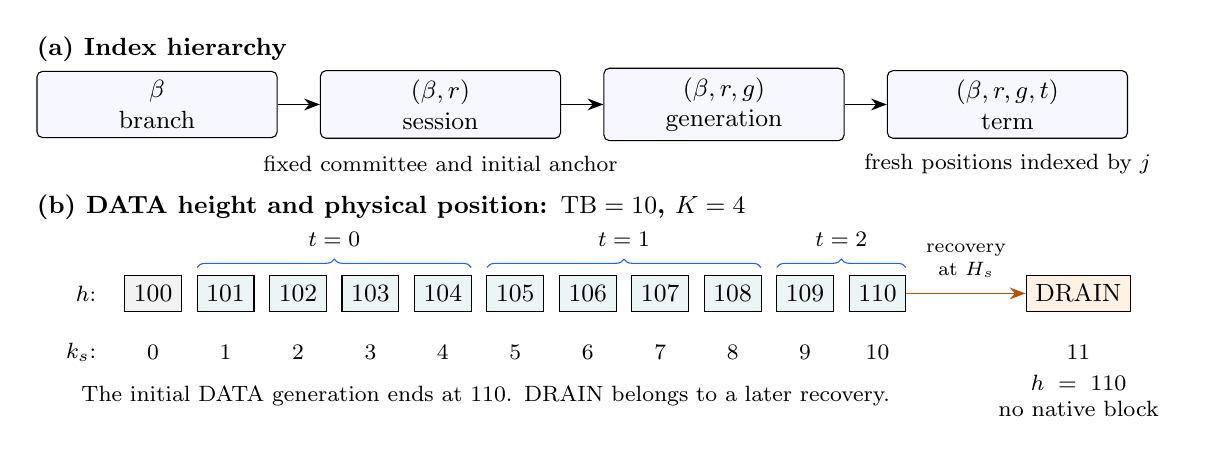
\begin{tikzpicture}[x=1cm,y=1cm,font=\small,
 box/.style={draw,rounded corners=2pt,minimum height=.65cm,
             minimum width=3.05cm,align=center,fill=blue!3},
 arr/.style={-{Stealth[length=2mm]},semithick}]
\node[anchor=west,font=\bfseries\small] at (0,3.05)
 {(a) Index hierarchy};
\node[box] (br) at (1.65,2.35) {$\beta$\\branch};
\node[box] (se) at (5.25,2.35) {$(\beta,r)$\\session};
\node[box] (ge) at (8.85,2.35) {$(\beta,r,g)$\\generation};
\node[box] (te) at (12.45,2.35) {$(\beta,r,g,t)$\\term};
\draw[arr] (br)--(se);\draw[arr] (se)--(ge);\draw[arr] (ge)--(te);
\node[align=center,font=\footnotesize] at (5.25,1.60)
 {fixed committee and initial anchor};
\node[align=center,font=\footnotesize] at (12.45,1.60)
 {fresh positions indexed by $j$};
\node[anchor=west,font=\bfseries\small] at (0,1.05)
 {(b) DATA height and physical position: $\TB=10$, $K=4$};
\node[anchor=east,font=\footnotesize] at (1.0,-.05) {$h$:};
\node[anchor=east,font=\footnotesize] at (1.0,-.80) {$k_s$:};
\node[draw,minimum width=.72cm,minimum height=.45cm,fill=black!5]
 (an) at (1.6,-.05) {100};
\node[font=\footnotesize] at (1.6,-.80) {0};
\foreach \i in {1,...,10}{
  \pgfmathsetmacro{\xx}{1.6+.92*\i}
  \pgfmathtruncatemacro{\hh}{100+\i}
  \node[draw,minimum width=.72cm,minimum height=.45cm,fill=teal!8]
   (b\i) at (\xx,-.05) {\hh};
  \node[font=\footnotesize] at (\xx,-.80) {\i};
}
\draw[decorate,decoration={brace,amplitude=3pt},draw=rrBlue]
 (2.16,.28)--(5.64,.28) node[midway,above=4pt,font=\footnotesize] {$t=0$};
\draw[decorate,decoration={brace,amplitude=3pt},draw=rrBlue]
 (5.84,.28)--(9.32,.28) node[midway,above=4pt,font=\footnotesize] {$t=1$};
\draw[decorate,decoration={brace,amplitude=3pt},draw=rrBlue]
 (9.52,.28)--(11.16,.28) node[midway,above=4pt,font=\footnotesize] {$t=2$};
\node[draw,minimum width=1.2cm,minimum height=.45cm,fill=orange!10]
 (dr) at (13.35,-.05) {DRAIN};
\node[font=\footnotesize] at (13.35,-.80) {11};
\node[font=\footnotesize,align=center,text width=2.5cm] at (13.35,-1.35)
 {$h=110$\\no native block};
\draw[arr,draw=rrOrange] (b10.east)--(dr.west)
 node[midway,above=2pt,font=\scriptsize,align=center] {recovery\\at $H_s$};
\node[font=\footnotesize,align=center,text width=10.2cm] at (5.8,-1.35)
 {The initial DATA generation ends at 110. DRAIN belongs to a later recovery.};
\end{tikzpicture}
\caption{Coordinates and quota. Panel (a) shows scopes, not a timing
trace. Panel (b) shows the initial generation's three DATA terms and a
possible later drain generation. The latter advances the physical
position but preserves the DATA height and executable state.}
\label{fig:indices-quota}
\end{figure}

\subsection{Signed messages, certificates, and admission}
\label{sec:objects-messages}

% P-3.07
Every signed regional message authenticates a canonical encoding of its
chain and rule version, message type, $\mathrm{cid}_s$, and typed payload.
The payload contains the session/view coordinates required by its type;
Table~\ref{tab:signed-messages} records the additional fields. All
validation uses the exact producing context. The block tuple in
Definition~\ref{def:regional-block} does not itself contain a plan or
$\mathrm{cid}$: those are bound by the signatures, not inferred from the
block hash alone.

\begin{table}[htbp]
\centering\small
\caption{Authenticated regional messages. Every row also binds the chain,
rule version, type, and session context. An opening identifies the exact
generation-opening block, including its height and physical position.}
\label{tab:signed-messages}
\begin{tabularx}{\linewidth}{@{}P{.21\linewidth}P{.20\linewidth}Y@{}}
\toprule
Type & Coordinates & Payload bound by the message\\\midrule
PROPOSE & $g,t,j$ & Generation opening; full block choice, including type,
$k,h$ and hash; parent justification.\\
DATA-VOTE / DRAIN-VOTE & $g,t,j$ & Generation opening, chosen block type,
$k,h$ and hash. Both types share one fresh-vote slot.\\
STATUS & $g,0$ & Fixed entry lock $Q_v$ and entry proof.\\
NEWVIEW & $g,0$ & Selected opening, justification $Q^*$ and entry proof.\\
ANCHOR-VOTE & $g,0$ & Selected recovery opening.\\
BLAME & $g,t$ & The admitted view; no opening, block hash, or local
progress count.\\
FINAL & $s,h(B)$ & Exact DATA hash. No generation or term field.\\
\bottomrule
\end{tabularx}
\end{table}

\begin{definition}[Regional certificate]
\label{def:regional-certificate}
A regional certificate consists of matching valid signatures from
\emph{distinct} members of $V_s$ whose total session weight is greater
than $F_s$. A proposal QC $\QC_{s,g,t}(B)$ certifies DATA-VOTE or
DRAIN-VOTE messages; an ANCHOR QC certifies the recovery opening; a BLAME
certificate certifies a view complaint; and a FINAL certificate
certifies a DATA hash under its session context. Repeated signatures by
one member contribute its weight only once.
\end{definition}
A correct member uses at most one fresh vote for a slot $(s,g,t,j)$,
including across DATA/DRAIN types, and at most one ANCHOR choice for a
recovery generation. Signatures are kept with their immutable slot
records. A QC establishes certified support, not expiration of a commit
timer. Neither assembling a QC nor casting an ANCHOR vote starts such a
timer. Since FINAL has no $g,t$ field, matching FINAL signatures on one
DATA may combine across generations of the same session, but not across
contexts or sessions.

% P-3.08
\paragraph{Anchors, openings, and justifications.}
The anchor $A_{s,g,t}$ precedes the fresh positions of its view. At
initial entry it is $A_s$; at recovery entry it is the selected opening
$A_{s,g,0}$; and for $t>0$ it is the preceding term's terminal DATA.
The inherited base justification $Q_s^0$ identifies exactly $A_s$ and
its original commitment evidence. If this evidence is a covering
receipt rooted at a later block, that root is evidence only: $Q_s^0$
still justifies $A_s$. For genesis or an L1-derived anchor, the
corresponding checkpoint or derivation evidence has the same base role.
It is not a new vote or QC from the entering committee.

Within one session, a proposal QC for $B$ has lexicographic rank
$(g,t,k_s(B))$. An ANCHOR QC has rank $(g,0,k_s(A_{s,g,0}))$, below the
first fresh QC of that recovery; $Q_s^0$ ranks below all own-session
QCs. A fixed order on certified block/opening identities breaks equal
ranks, independently of signature-set encodings. The opening identity
is $(g,k_s(A_{s,g,0}),h(A_{s,g,0}),\Hash(A_{s,g,0}))$.
$Q_v$ denotes a replica's entry lock, fixed when it enters a recovery
generation, and $Q^*$ the leader's selected justification. Ranks are
compared only within the session; a foreign session's QC cannot replace
$Q_s^0$ or become an own-session entry lock.

\begin{table}[htbp]
\centering\small
\caption{Parent and justification for a fresh proposal. The recovery row
also applies to a drain generation, including one whose opening is an
older DRAIN. No rule requires the parent to be committed before proposing.}
\label{tab:parent-rule}
\begin{tabularx}{\linewidth}{@{}P{.22\linewidth}Y Y@{}}
\toprule
Case & Parent block & Required justification\\\midrule
$g=t=j=0$ & Fixed initial anchor $A_s$ & $Q_s^0$.\\
$g>0$, $t=j=0$ & Recovery opening $A_{s,g,0}$ & Its ANCHOR QC in the
current generation.\\
$j=0$, $t>0$ & Terminal DATA of term $t-1$ & Its proposal QC in that
preceding term.\\
$1\le j<m_{s,g,t}$ & Fresh block at $j-1$ of the same term & Its proposal
QC in the same view.\\
\bottomrule
\end{tabularx}
\end{table}

% P-3.09
\begin{definition}[Admission and complete Quit evidence]
\label{def:admission-quit}
Initial view $(s,0,0)$ is admitted by guarded Enter using its fixed
handoff. A recovery view $(s,g,0)$, $g>0$, requires the preceding
complete Quit proof and finalized $\mathsf{REC}(\mathrm{cid}_s,g)$.
A later term additionally requires the terminal QCs of its preceding
terms, each for DATA below $H_s$. For remote verification, the
\emph{admission witness} supplies the corresponding boundary, recovery
entry proofs and authority records, and terminal-QC ancestry.
A view message is \emph{admissible} when its view is admitted, its
signed context and generation match, and its required signatures are
valid under that context. Leader-signed messages must be signed by
$L(\beta,r,g,t)$ for that exact view.
A complete Quit proof for an admitted generation is one of:
\begin{enumerate}[label=(\alph*)]
\item a BLAME certificate for an admitted term, with that term's
admission witness;
\item two different admissible DATA or DRAIN proposals signed by the
designated leader at the same $(s,g,t,j)$, with the material needed to
check their admission and quota; or
\item for $g>0$, two valid NEWVIEW messages from its designated recovery
leader selecting different opening blocks.
\end{enumerate}
\end{definition}
Different openings conflict even when one extends the other; different
QC encodings for the \emph{same} opening do not constitute that conflict.
An over-quota DATA or a DRAIN outside a drain generation is not an
admissible proposal for case (b). A silent leader does not postpone
admission of its term or the start of its progress checks.

Complete regional validation checks the signatures and authority,
admission, type, quota, both positions, references, parent rule and
justifications, hash links, and native input validity over the required
ancestry. It uses actual block bodies and verified source records,
rather than only their names or hashes. Regional replicas perform this
validation before their own protocol actions. The Authority's relative
checks use the claimed context's fixed sources and signed slots; they
do not establish canonical handoff history or execute the global rule.
The public FINAL kernel is a separate check whose soundness must be
proved from actual correct signing and commit events, not assumed as
part of raw signature verification.

\subsection{Handoffs, readiness, and regional results}
\label{sec:objects-handoffs}

% P-3.10
\begin{definition}[Handoff descriptor]
\label{def:handoff}
A selected session has descriptor
\[
 \nu=(\beta,r,i,A,H,q^{\rm open},\mathit{cause},\Pi),
 \qquad i=\mathsf{region}(\Pi),\quad H=h(A)+\TB.
\]
Its cause is GENESIS, REGULAR, FORCE$(c,q_f)$, or
RESUME$(c,p_{\rm eff})$. Here $c$ is the unique L1 control sequence
number, $q_f$ is the ordinary Force's Espresso activation height, and
$p_{\rm eff}=(\ell,txIndex,logIndex)$ is the finalized L1 position of
the corresponding ModeApplied event. A complete handoff additionally supplies the
branch policy, the selection reference and source region used by the
plan, the L1 bound
\[
 \lambda_s^{\rm open}=\max\{\lambda(A_s),\lambda(\Pi_s)\},
\]
and the evidence fixing these fields and $Q_s^0$.
An unassigned boundary is
\[
 \omega=(\mathit{cause},\beta,r,i_{\rm src},A,q^{\rm open});
\]
it has a fixed target pair and anchor but no selected region.
\end{definition}
A regular handoff fixes $A_{s'}=T_s$, $E_{s'}=A_s$, and
\begin{equation}
\label{eq:regular-reference-floor}
 q_{s'}^{\rm open}=
 \max\{\operatorname{height}(\xi(T_s)),q_s^{\rm open}+1\}.
\end{equation}
Its evidence includes the authentic predecessor boundary and complete
terminal result. A Force handoff uses the exact retained global tip
and its activated control; a resumed handoff uses the actual derived
terminal state of the deposit-only interval and its committed mode
boundary. Their public replay fixes the target pair, source region and
reference floors. Neither the receiver's current local tip nor a
sender's claimed highest production determines these fields. The
inherited anchor retains its original producer or L1 provenance.

Historical handoff verification and current entry permission are
separate predicates. Historical verification reconstructs the fixed
fields from an authorized checkpoint and the complete relevant source
history. Current permission additionally requires the assigned member,
a current version not marked closed in the node's verified history,
and a pair that has not already entered or terminated. The same test
applies if the first received ReadyBundle would create the local
instance. A later source record cannot replace a previously fixed
handoff for the same pair with different fields.

% P-3.11
\begin{definition}[Ready]
\label{def:ready}
An Assigned instance for $s$ is \emph{Ready} when:
\begin{enumerate}[label=(\roman*)]
\item its handoff has been authenticated and current entry permission
holds;
\item the exact anchor, its original identity, required ancestry and
commitment or derivation evidence have been validated;
\item the node holds a validated, directly usable executable state
$\mathit{st}(A_s)$, with no remaining reconstruction or installation
work; and
\item its plan, policy, quota and reference floors, with their required
source records, are available and validated.
\end{enumerate}
\end{definition}
A ReadyBundle carries that handoff, full anchor/evidence material,
executable state and its native validation evidence, and the required
source records. It carries no inherited locks, votes or timers.
Recipients verify its contents and may reuse local state only when it
is the state after the same exact anchor. A state root, URL, or promise
to fetch later is insufficient. The header at $q_s^{\rm open}$ need not
yet exist for Ready or initial Enter; the first DATA must wait until
its own reference condition is satisfiable. ReadyBundle is a delivery
object, not a READY quorum certificate, and a duplicate does not reset
entry time.

% P-3.12
\begin{definition}[Regional FINAL receipt and complete result]
\label{def:regional-result}
Let $C_s$ be an authentic producing context. A direct regional FINAL
receipt $\FC_s(B)$ consists of matching FINAL signatures on the exact
DATA block $B$ of $s$ from distinct members of weight greater than $F_s$;
$B$ extends
$A_s$, lies within its session's quota, and has intrinsically valid
regional ancestry under that context. A covering receipt for $B$ is a
valid direct receipt on a same-session DATA descendant $D$, together
with the exact validated ancestry from $D$ to $B$.
A complete regional result contains the target DATA, the direct or
covering receipt with its full bodies, and the historical context and
source material needed for the consumer's specified validation.
\end{definition}
The reusable public kernel for a target is $(D,\Sigma,\pi)$: root DATA,
FINAL signatures on that root, and the full hash-linked path to the
target. Direct evidence takes $D=B$. Its raw threshold test checks only
the exact signed context, DATA identity and weight; it does not assume
the intrinsic validity claimed in Definition~\ref{def:regional-result}.
The later public-check argument establishes that validity through a
correct signer. Regional full validation additionally uses the actual
proposals, QCs, admission witnesses and finalized Authority records
that its own actions require; these objects do not become mandatory
sidecars of the public kernel merely because a publisher attaches them.

A correct replica emits a new FINAL only when a commit-timer event
commits the DATA directly or as an ancestor. A receipt-induced commit,
including Completion, emits no new FINAL. A DRAIN timer may cause FINAL
for the terminal DATA, never for the DRAIN itself. A successor never
re-signs its inherited anchor under its new committee. Coverage never
crosses sessions: a successor's receipt cannot replace the predecessor's
terminal evidence. A complete receipt may support a regular handoff
before it supports any global append. Regional finality is therefore a
statement about a specified, authenticated production ancestry; it is
not a claim that the ancestry has been selected into $G$.

\subsection{State ownership and invocation rules}
\label{sec:objects-state}

% P-3.13
\begin{table}[htbp]
\centering\small
\caption{State ownership. Immutable validated objects may be shared;
mutable consensus state belongs to exactly one local session instance.}
\label{tab:state-ownership}
\begin{tabularx}{\linewidth}{@{}P{.21\linewidth}Y@{}}
\toprule
Owner & Authoritative local or ledger state\\\midrule
L1 Authority & Positions and escrow, frozen epoch tables, ban history,
REC, processed offenses, control log and clearance/release records.\\
Session Program & Fixed context and endpoint; current view, individual
signing slots, locks, votes, QCs, timers, commitments and execution state.\\
Session Manager & Handoffs, entry/termination records, Closed versions,
production branch $R$, replay state for $G$, and exact prepared anchors.\\
Publisher & Complete-result store, deduplication identifiers, durable
pending sends and publication progress.\\
Batcher/inbox & Local channel construction and, separately, L1-accepted
frame/block progress and committed mode boundaries.\\
Trusted certifier & Validated source/replay state and its typed business
conclusions; no authority to invent a different protocol interpretation.\\
Derivation node & Actual native head and state, consumed L1 positions,
accepted channel data, mode state and pending input dependencies.\\
\bottomrule
\end{tabularx}
\end{table}
The Session Manager follows the global chain $G$ and a possibly longer
regional production branch $R$. It keeps a baseline state at
$\operatorname{last}(G)$ and may prepare a regular successor at a later
regionally finalized anchor. Each Program receives the state of its
own exact anchor. Subsequent baseline progress does not change that
Program's starting point. A shared PublicStore retains authenticated
source bytes, regional evidence, checkpoints and outstanding delivery
tasks independently of Program lifetime. Closing an instance removes
its permission to act, not the obligation to retain or transfer data.

For public replay, $\mathsf{NEXT}(\nu)$ identifies a selected next-block
owner; $\mathsf{PENDING}(\omega)$ records a boundary whose complete plan
selects no region. $\mathsf{OPEN}(\omega,E)$ records fixed inputs whose
plan is not yet available, and $\mathsf{DEPOSIT}$ carries the committed
L1-mode continuation state. OPEN is a transient evidence wait, not a
third production mode. The two modes remain NORMAL and DEPOSIT\_ONLY.
The global rule and derivation rule are deterministic computations
performed by their consumers, not additional consensus services.

% P-3.14
\paragraph{Results, errors, and durable effects.}
A successful query returns a value. \textsf{WAIT} identifies unavailable
required information and leaves the caller at its saved operation;
\textsf{REJECT} rejects a decidably invalid request without its proposed
state change. A verified $\bot$ or empty set is a result obtained from
complete evidence, not a substitute for a failed fetch.
\textsf{INCONSISTENT} is reserved for contradictory authenticated
canonical inputs or a violated continuation invariant; unverified
network garbage cannot trigger it merely by asserting a competing
boundary. A paused caller preserves already committed output and
resumes from its durable execution position.

An authenticated L1 call binds its caller, stable request identifier,
chain, version and arguments; repeated identifiers with identical
content return the recorded result, while conflicting reuse is rejected.
Consensus and publication objects have their own stable content and
slot identities. Changing a QC's signer set or proof encoding does not
create a new block choice or restart a vote timer. State changes, signed
slot records, execution positions and pending outgoing actions are
persisted before dispatch. Retransmission may repeat bytes but not the
logical action. Inputs contain the exact required bodies and source
records, or references that the receiver can resolve within the claimed
processing budget. These conventions apply to every later protocol
block and to the detailed internal interfaces.

\end{document}
